\documentclass[12pt]{report}

% Use utf-8 encoding for foreign characters
%\usepackage[utf8]{inputenc}
%\usepackage{fullpage}
%\pdfpagewidth 8.5in
%\pdfpageheight 11in

% Uncomment some of the following if you use the features
%
% Running Headers and footers
\usepackage{fancyhdr}
\pagestyle{fancy}
\fancyhf{}
\setlength{\headheight}{1.5 ex}
\setlength{\headsep}{1.5 ex}

% Multipart figures
%\usepackage{subfigure}

% More symbols
\usepackage{amsmath}
\usepackage{amssymb}
\usepackage{latexsym}

% Surround parts of graphics with box
\usepackage{boxedminipage}

% This is now the recommended way for checking for PDFLaTeX:
\usepackage{ifpdf}

\ifpdf
\usepackage[pdftex]{graphicx}
\else
\usepackage{graphicx}
\fi


\title{RateMyCourses: A Collaborative Course Evaluation Environment}
\author{Stephen Gelman \and Ravi Kotecha \and Andrew Lewis \and Kevin Weaver}
\date{5 March 2010}

\newcommand{\HRule}{\rule{\linewidth}{0.5mm}}

\begin{document}
\thispagestyle{plain}

\fancyhead[LE,LO]{Gelman, Kotecha, Lewis, Weaver}
\fancyhead[RE,RO]{RateMyCourses}
\fancyfoot[C]{\thepage}

\ifpdf
\DeclareGraphicsExtensions{.pdf, .jpg, .tif, .png}
\else
\DeclareGraphicsExtensions{.eps, .jpg}
\fi

\begin{titlepage}
 
\begin{center}
 
\textsc{\LARGE COSI 125a: Human-Computer Interaction}\\[1.5cm]
 
\textsc{\Large Term Project}\\[0.5cm]
 
 
% Title
\HRule \\[0.4cm]
{ \huge \bfseries RateMyCourses}\\[0.4cm]
{\bfseries A Collaborative Course Evaluation Environment}
 
\HRule \\[1.5cm]
 
% Author and supervisor
\begin{minipage}{0.4\textwidth}
\begin{flushleft} \large
\emph{Authors:}\\
Stephen \textsc{Gelman}\\
Ravi \textsc{Kotecha}\\
Andrew \textsc{Lewis}\\
Kevin \textsc{Weaver}\\
\end{flushleft}
\end{minipage}
\begin{minipage}{0.4\textwidth}
\begin{flushright} \large
\emph{Professor:} \\
Richard \textsc{Alterman}\\
\bigskip
\emph{Teaching Assistant:} \\
Alex \textsc{Gaman}\\
\end{flushright}
\end{minipage}

\vfill

Prototype 1: \texttt{http://ratemycourses-dev.brandeis.edu}

Prototype 2: \texttt{http://ratemycourses.brandeis.edu}
 
\vfill
 
% Bottom of the page
{\large 5 May 2010}
 
\end{center}
 
\end{titlepage}


\begin{abstract}
In this paper we present RateMyCourses, a collaborative course evaluation and social tagging environment. The aim of the site is to fully develop an asynchronous collaborative knowledge community based on collective experiences of students in the classroom. The scope of this utility is within Brandeis University and includes students, faculty, staff, and administrators. In the design of RateMyCourses we have taken a user-centric approach. We design iteratively, seeking frequent user feedback. Here we outline, in detail, the design process and analysis during and after the development of RateMyCourses 2.0. Finally, we identify both strong and weak points in our interface design and enumerate several areas that can be improved upon in the future.
\end{abstract}

\tableofcontents

\chapter{Introduction}

For our term project this semester we built upon the RateMyCourses (RMC) system developed by Andy Lewis, Ravi Kotecha, and Stephen Gelman in CS118.  We added Kevin Weaver to the development team this semester to build upon the prototype we developed last year. RMC is a collaborative course evaluation and social tagging environment. The aim of this site is to fully develop an asynchronous collaborative knowledge community based on collective experiences of students in the classroom. This website builds relationships between courses across academic departments by linking classes with tags through keywords. Courses can also be directly linked to one another, something we call ``Cross-linking.'' The scope of this utility is within Brandeis University and includes students, faculty, staff, and administrators. People who use the website can see all the courses offered at Brandeis and tag them with various tags relating to the courses, such as ``Writing Intensive'', ``Lots of Work'', etc. Tags can also relate to course topics, providing the ability to match up similar courses between departments. Students are also offered the opportunity to rate courses they have taken. Also, similar to sites like Amazon.com, RMC will keep track of what users have rated and display a box similar to ``Students who took this course also took...'' so that students can find similar courses. Our goal with this project is to give students a better idea of the courses offered at Brandeis and to enable them to know more about the content and quality of a class going into it.

\section{Current Approaches}

Brandeis currently provides two ways to search for classes. The first is through the Registrar website, which filters the course schedule by subject, description keyword, requirement, and class meeting time. The second method is through the Student Union's Course Evaluation Guide. Brandeis currently collects surveys from students at the end of each semester. The surveys rate different aspects of each course, such as, the overall quality, the professor's attentiveness, and the difficulty. At the end of each year, a student is hired to analyze the data and compile summaries and reviews of each of the courses. This method works if students would like to read a summary of a given course during a specific semester. However, the either system does not allow for easy browsing and there is no sort of tagging to allow a student to find similar courses from different departments. The two websites to browse for courses are the Registrar search (http://www.brandeis.edu/registrar/schedule/search) and the Course Evaluation Guide (https://sys.brandeis.edu/ceg/index).

The system we built allows members of the Brandeis community to explore the course curriculum in a new, innovative way based on collaborative tagging. This tool is designed to facilitate course selection and provide students the ability to find classes in different departments based on their interests that they would not have been able to find otherwise.

Though functionality is important to the system, a key component of the website is the interface design.  As we have learned in our class, interfaces must be user-oriented in order for people to easily use the website. Additionally, the design process must be a cycle which incorporates end-user feedback throughout the process. Throughout this project lifecycle, we iteratively developed two prototypes, consulting with end-users both during and after development of each. We interviewed users and collected responses, which helped shape the design. After the development of the second prototype, we further applied principles we learned in class, critiquing the interface based on the principles of Norman, Schneiderman, and Nielson and conducting a GOMS analysis on our design.

\section{Implementation Details}

As with version 1.0, we programmed RateMyCourses using a Python web framework called TurboGears.  TurboGears uses the Model-View-Controller pattern of software engineering.  This means that the data storage aspect is separated from the backend code which is, in turn, separated from the templates that the user sees.  The advantage of this separation is that it is easy to change one piece of the application without having to modify everything.  This was very useful when we were receiving feedback from people because it made it easy to change the design of the site without having to rewrite much code other than HTML.

The login for the site uses Brandeis' Cosign SSO for authentication (viewable through: http://login.brandeis.edu).  The advantage of this is that users can log in with their UNET IDs and passwords.  This is useful because it prevents the user from having to register their usernames.  The downside to this was that it prevented users from choosing anonymous usernames because most users' UNET IDs are some permutation of their real name or searchable in the Brandeis People Directory.  To counter this we added the ability for a user to set an anonymous alias.  The advantage of this is that it gives users pseudo-anonymity, but at the same time if a user posts a disparaging comment an administrator can look up who they actually are.


\chapter{User Analysis}

\section{User Profiles}
Our potential users are students, faculty, staff and administrators of Brandeis University. We determined the needs and requirements of users by a combination of informal interviews and observations, and set upon developing the following user profiles and tasks which cover the majority of users of our system.

\begin{tabular}{|l|p{8cm}|}
\hline
\textbf{User type:}	& Advanced User ``Alice''\\
\hline
\textbf{User description:}	& Alice has used RMC before and understands the usefulness of user-defined tags. \\
\hline
\textbf{Use case scenario:}	& Alice has recently completed a course, ``COSI 125a: Human-Computer Interaction''. She recalls that it was a fun course, but it required a lot of reading, and she wants future students to know. \\
\hline
\textbf{User Tasks:}	&  Alice knows that a tag called ``FunClass'' already exists, so she selects it from the ``Add Tag'' menu. She then proceeds to type the word ``reading'' into the ``New Tag'' text input field. To her surprise, the tag ``LotsOfReading'' already exists and autocompletes as she types. The two new tags appear on the course page immediately after they are added. \\
\hline
\textbf{Needs: }	& Must be able to define a new tag. Must be able to search for existing user-defined tags. \\
\hline
\end{tabular}

\bigskip

\begin{tabular}{|l|p{8cm}|}
\hline
\textbf{User type:}	&  Novice User ``Bob''\\
\hline
\textbf{User description:}	&  Bob is less likely to add a tag to a course himself, but he understands the usefulness of tags. \\
\hline
\textbf{Use case scenario:}	&  Bob logs in to RMC and finds the course page for COSI 125a. He agrees that it was a fun course, but found the amount of reading to be quite reasonable, so he disagrees with Alice's choice of the ``LotsOfReading'' tag. \\
\hline
\textbf{User Tasks:}	&  Bob upvotes the ``FunClass'' tag and downvotes the ``LotsOfReading'' tag by clicking the corresponding arrows next to the tag text. \\
\hline
\textbf{Needs: }	& Must be able to vote on the usefulness of a user-defined tag.\\
\hline
\end{tabular}

\bigskip

\begin{tabular}{|l|p{8cm}|}
\hline
\textbf{User type:}	&  New User ``Carol''\\
\hline
\textbf{User description:}	&  Carol has just started to use RMC and has few preconceived notions about tagging in general. \\
\hline
\textbf{Use case scenario:}	&  Carol is looking for a fun course to take in the Computer Science department. \\
\hline
\textbf{User Tasks:}	&  Carol logs into RMC and enters ``Computer Science fun'' into the search bar at the top of the page. In addition to the tags ``ComputerScience'' and ``FunClass'', the search reveals a list of courses that contain both of these tags.\\
\hline
\textbf{Needs: }	& Must be able to do a keyword-based search for a course. Must be able to understand the usefulness of tags at a glance.\\
\hline
\end{tabular}

\bigskip

\begin{tabular}{|l|p{8cm}|}
\hline
\textbf{User type:}	&  New User ``Dennis''\\
\hline
\textbf{User description:}	&  Dennis is not exceptionally computer-savvy, but also dislikes reading directions. \\
\hline
\textbf{Use case scenario:}	&  Dennis has just logged into RMC for the first time and is unsure of where to start. \\
\hline
\textbf{User Tasks:}	& On the home page, Dennis follows the tutorial for first time users. This provides a nice visual walkthrough with accompanying text. Dennis does so, learning how to search for and tag courses in the process. \\
\hline
\textbf{Needs: }	& Must be able to know what to do upon logging in for the first time. Must be able to quickly learn how to rate and tag courses.
\\
\hline
\end{tabular}

\bigskip

\begin{tabular}{|l|p{8cm}|}
\hline
\textbf{User type:}	&  Experienced User ``Emily''\\
\hline
\textbf{User description:}	&  Emily has used RMC before and has rated a few courses. She has not necessarily tagged any courses or voted on any tags. \\
\hline
\textbf{Use case scenario:}	&  Emily intends to log in to RMC today to find some courses for the next semester that might interest her. \\
\hline
\textbf{User Tasks:}	&  After logging in to RMC, Emily notices a message at the top of the page listing a few courses that she might enjoy based on her previous ratings. \\
\hline
\textbf{Needs: }	& Must be able to find recommendations for courses to take in the future. \\
\hline
\end{tabular}

\section{Requirements}

Based on these tasks, we identified the following requirements:

\begin{tabular}{|l|p{7.5cm}|}
\hline
\textbf{Requirement id:}	& 1 \\
\hline
\textbf{Requirement name:}	&  Define New Tag \\
\hline
\textbf{Requirement type:}	& Functional \\
\hline
\textbf{Description:}	&  Users must be able to define new tags and apply them to courses. \\
\hline
\textbf{Rationale:}	&  RMC is built around the idea of folksonomy tagging, which requires giving users the power to create new tags. \\
\hline
\textbf{Source:}	& User \\
\hline
\textbf{Dependencies:}	& None \\
\hline
\textbf{Conflicts:}	& None \\
\hline
\textbf{Supporting materials:}	& None \\
\hline
\end{tabular}

\bigskip

\begin{tabular}{|l|p{7.5cm}|}
\hline
\textbf{Requirement id:}	& 2 \\
\hline
\textbf{Requirement name:}	&  Search for Tag \\
\hline
\textbf{Requirement type:}	& Functional \\
\hline
\textbf{Description:}	&  Users must be able to search for previously-defined tags with ease. \\
\hline
\textbf{Rationale:}	& In order to avoid defining redundant tags, users should be able to search for and quickly identify tags and tag definitions that may fit their needs. \\
\hline
\textbf{Source:}	& User \\
\hline
\textbf{Dependencies:}	& None \\
\hline
\textbf{Conflicts:}	& None \\
\hline
\textbf{Supporting materials:}	& None \\
\hline
\end{tabular}

\bigskip

\begin{tabular}{|l|p{7.5cm}|}
\hline
\textbf{Requirement id:}	& 3 \\
\hline
\textbf{Requirement name:}	&  Vote on Course Tag \\
\hline
\textbf{Requirement type:}	& Functional \\
\hline
\textbf{Description:}	&  Users must be able to vote on the usefulness of a user-defined tag for a given course. \\
\hline
\textbf{Rationale:}	&  Because any user can apply any tag to any course, there needs to be a way to democratically determine the tag's appropriateness and usefulness. \\
\hline
\textbf{Source:}	& User \\
\hline
\textbf{Dependencies:}	& None \\
\hline
\textbf{Conflicts:}	& None \\
\hline
\textbf{Supporting materials:}	& None \\
\hline
\end{tabular}

\bigskip

\begin{tabular}{|l|p{7.5cm}|}
\hline
\textbf{Requirement id:}	& 4 \\
\hline
\textbf{Requirement name:}	&  Search for Course \\
\hline
\textbf{Requirement type:}	& Functional \\
\hline
\textbf{Description:}	&  A user must be able to quickly search for a course based on the course name, description, or tags. \\
\hline
\textbf{Rationale:}	&  Users will not be willing to spend a long time searching for a particular course in order to rate or tag it. \\
\hline
\textbf{Source:}	& User \\
\hline
\textbf{Dependencies:}	& None \\
\hline
\textbf{Conflicts:}	& None \\
\hline
\textbf{Supporting materials:}	& None \\
\hline
\end{tabular}

\bigskip

\begin{tabular}{|l|p{7.5cm}|}
\hline
\textbf{Requirement id:}	& 5 \\
\hline
\textbf{Requirement name:}	&  Understanding Tagging \\
\hline
\textbf{Requirement type:}	& Usability \\
\hline
\textbf{Description:}	&  New users must be able to quickly understand the usefulness of tags. \\
\hline
\textbf{Rationale:}	&  Without a decent understanding of folksonomy tagging, a user cannot properly evaluate a given course, and the site is rendered useless. \\
\hline
\textbf{Source:}	& User \\
\hline
\textbf{Dependencies:}	& None \\
\hline
\textbf{Conflicts:}	& None \\
\hline
\textbf{Supporting materials:}	& None \\
\hline
\end{tabular}

\bigskip

\begin{tabular}{|l|p{7.5cm}|}
\hline
\textbf{Requirement id:}	& 6 \\
\hline
\textbf{Requirement name:}	&  New User Orientation \\
\hline
\textbf{Requirement type:}	& Usability \\
\hline
\textbf{Description:}	&  A new user must be unobtrusively guided through the site. \\
\hline
\textbf{Rationale:}	&  A user should not be forced to explore the site in order to learn how it works. New users should be gently guided through rating and tagging their first courses in order to help them develop an understanding of RMC. \\
\hline
\textbf{Source:}	& User \\
\hline
\textbf{Dependencies:}	& None \\
\hline
\textbf{Conflicts:}	& None \\
\hline
\textbf{Supporting materials:}	& None \\
\hline
\end{tabular}

\bigskip

\begin{tabular}{|l|p{7.5cm}|}
\hline
\textbf{Requirement id:}	& 7 \\
\hline
\textbf{Requirement name:}	&  Course Recommendations \\
\hline
\textbf{Requirement type:}	& Functional \\
\hline
\textbf{Description:}	&  A user must be able to see recommendations for courses to take based on past ratings. \\
\hline
\textbf{Rationale:}	&  The usefulness of RMC is based on its ability to assist users in finding interesting courses. A recommendation engine would take some of that work out of the users' hands and give them an incentive to continue rating and tagging courses. \\
\hline
\textbf{Source:}	& User \\
\hline
\textbf{Dependencies:}	& None \\
\hline
\textbf{Conflicts:}	& None \\
\hline
\textbf{Supporting materials:}	& None \\
\hline
\end{tabular}

\section{Task Analysis}

We created a hierarchical task analysis for our tasks which helped determine the design and layout.

Hierarchical task analysis for Task-1:  Define New Tag
\begin{enumerate}
\item Go to a specific course page
\item Click ``Add Tag''
\item Choose tag from list OR define new tag with description 
\end{enumerate}

Hierarchical task analysis for Task-2: Search for Tag
\begin{enumerate}
\item Enter keyword into search box
\item Hit return key
\item View results 
\end{enumerate}

Hierarchical task analysis for Task-3: Vote on Course Tag
\begin{enumerate}
\item Go to a specific course page
\item Click thumbs up or thumbs down button next to tag 
\end{enumerate}

Hierarchical task analysis for Task-4: Search for Course
\begin{enumerate}
\item Enter keyword into search box
\item Hit return key
\item View results 
\end{enumerate}


\chapter{Conceptual Model and Interaction Style}

Like many social bookmarking sites, the underlying conceptual model of RateMyCourses is a large, directed graph representing relationships between different nodes. The three main node types are courses, ratings, and tags.

Course nodes are created by the system via feeds from the Registrar. These nodes are static and are not modifiable by users, so the interface must clearly convey this lack of affordance. Courses must be easily searched by users; for this, we provide a simple keyword-based search, as well as a more advanced tag-based search.

Rating nodes are directed at a single course. These nodes are created by users who give a course a rating on a five-star scale. While a rating applies to a particular course, a single course may have many ratings by many different users. These are aggregated into a single average rating for the course, which is displayed on a five-star scale at the top of the course page. However, at the moment we do not clearly convey how many ratings have been applied to a single course, and it is not immediately clear that the star rating shown is an average rating.

Tags can be directed at many courses. These nodes are separated into two categories: system tags and user-defined tags. System tags are used to indicate university requirements, major requirements, and other course attributes defined by the Registrar; they cannot be modified by users. User-defined tags are folksonomy tags that are used to describe more qualitative attributes of a course. These tags are not separated stylistically, but are instead separated spatially on individual course pages. System tags are listed under the course title and are surrounded by horizontal rules, whereas user-defined tags are listed under the course description and are followed by an ``Add Tag'' link. The rationale behind the spatial but not stylistic separation is to make it clear that all tags can be used to find courses, but some tags cannot be modified.

Additionally, we have implemented vertices known as ``crosslinks'' that connect different course nodes. This allows users to link two similar courses without the need to create a new tag and apply it to both courses.


\chapter{Design Process}

At the beginning of the planning process, we met several times to discuss potential stakeholders. We determined that potential users would include primarily students, but also faculty advisers and department administrators. Because this was a continuation of a previous project, we had the advantage of using existing user data from our first prototype. After making a few mainly aesthetic changes to the original site, we carried out several unstructured interviews to get a better idea of what users were looking for. Additionally, we imagined some scenarios based around several typical user profiles and listed a number of needs and requirements that we would need to act on during development.

Using this data, we developed a second prototype that attempted to address several concerns users had about the first prototype, mainly the way courses were searched for and the way different tags were presented and distinguished from one another. We also decided, based on time constraints, to eliminate some features and ideas that we had, and chose rather to focus on a small subset of features but develop them as best we could. We performed a GOMS analysis on the new prototype in an attempt to identify ways to reduce memory load when searching for and tagging courses.

Once our second prototype was completed, we developed a short survey and distributed it to a wide audience with the intention of soliciting feedback on users' first impressions of the new interface. We also interviewed a few more people using the same questions from the first interview so that we could identify what aspects were improved and where things had become more confusing.


\chapter{Prototype 2 Task Narrative}

\section{Defining a new tag and adding a tag}

To define a new tag, the user first logs in.  Then, they find a course they would like to tag either via searching or browsing the course list.  From the course page, they click the ``Add Tag'' button, which pops up the window in Figure~\ref{fig:add-tag}. From that window, the user has two choices.  First, they can type a tag into the text box.  As the user types, the box will attempt to autocomplete from the list of tags already in the system.  If the user enters a tag that does not exist the tag is added to the system when they click ``Add Tag''.  Alternatively, the user can click on a tag in the list of tags to add it to the course.

\begin{figure}
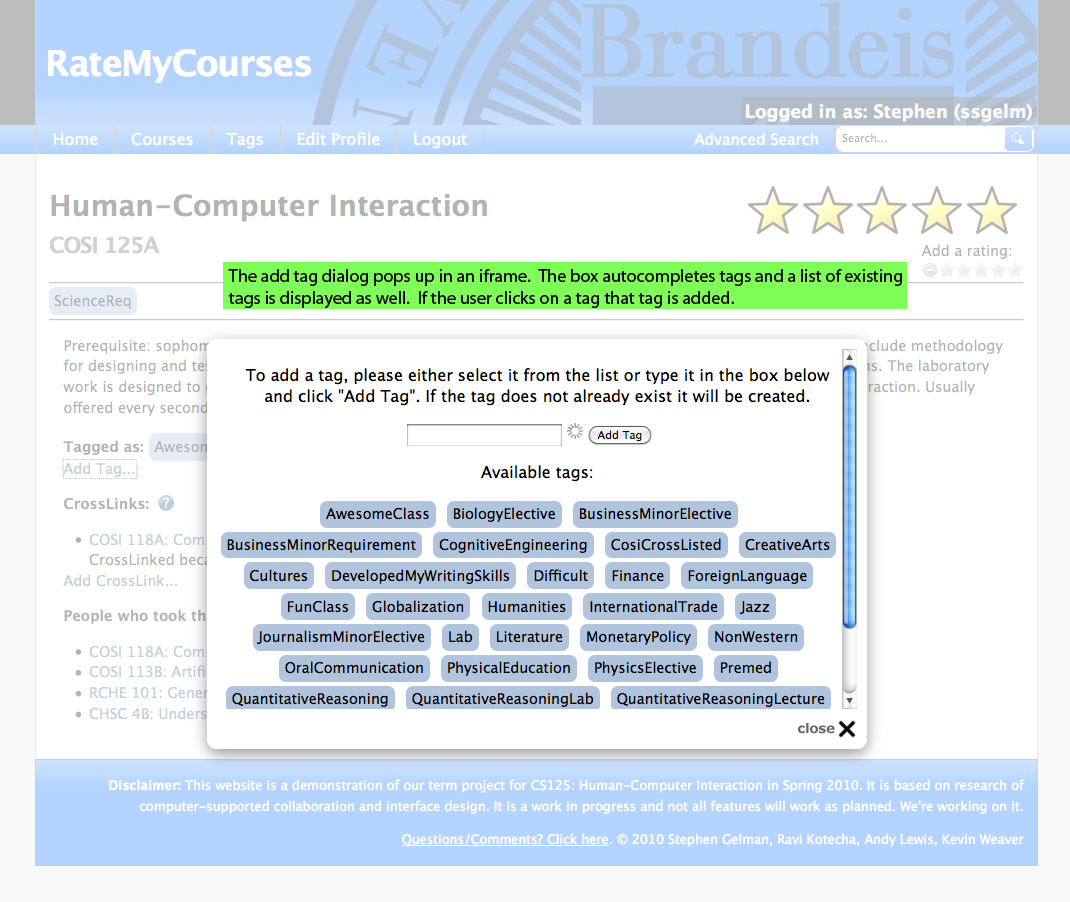
\includegraphics[width=\textwidth]{narrative-1.png}
\caption{Adding a tag}
\label{fig:add-tag}
\end{figure}

\section{Searching for a course}

There are two ways that the user can find a course.  One way is by using the search box.  If the user types part of a course name in the search box in the upper-right corner of the page, the system will display a page as in Figure~\ref{fig:search-keyword}. The user can then select a course from that list.  Alternatively, the user can click the ``Courses'' link at the top of the screen to browse for a course.  The course browsing page is a tree view that separates the courses by subject (see Figure~\ref{fig:search-treeview}). Clicking on a ``folder'' for a subject expands it and shows the courses within it.  Then, clicking on a course name brings the user to the course page.

\begin{figure}
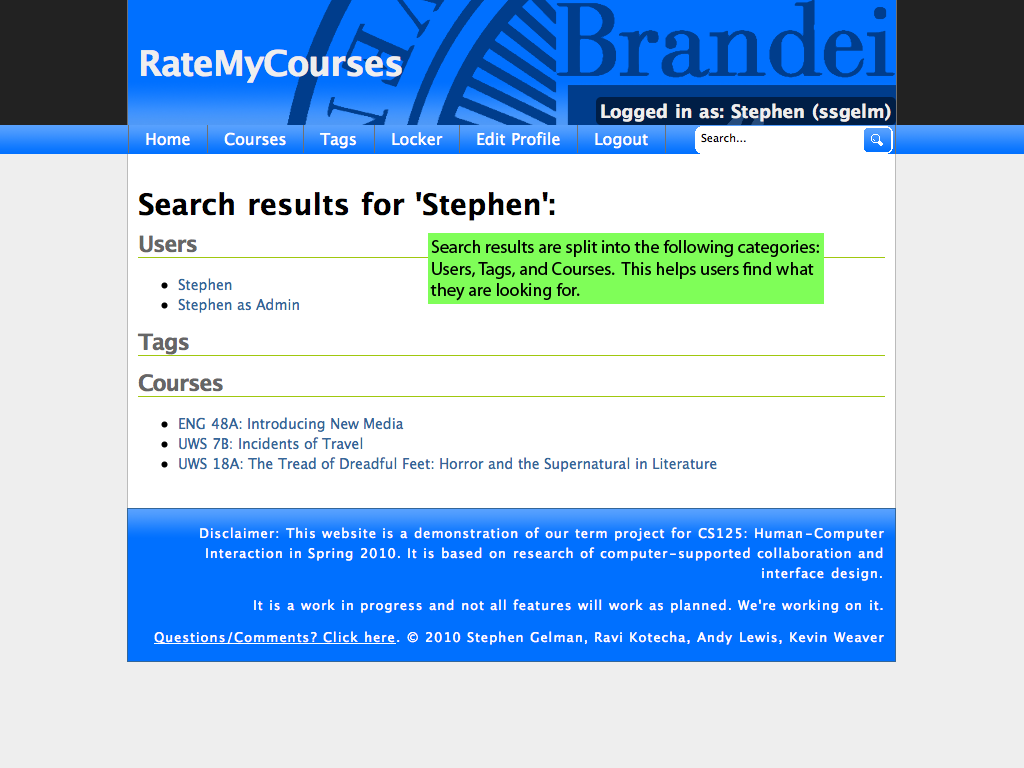
\includegraphics[width=\textwidth]{narrative-2.png}
\caption{Searching by keyword}
\label{fig:search-keyword}
\end{figure}

\begin{figure}
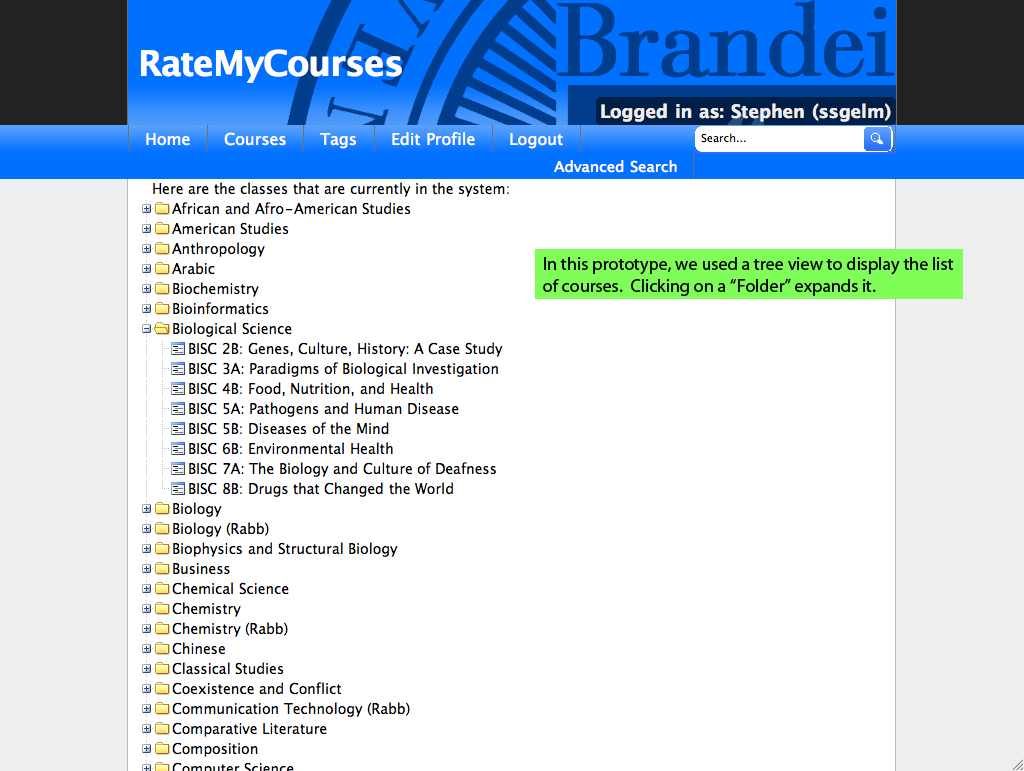
\includegraphics[width=\textwidth]{narrative-3.png}
\caption{Searching by hierarchical treeview}
\label{fig:search-treeview}
\end{figure}

\section{Voting on a course}

Voting is done from the course page.  To vote, a user clicks on the up or down arrows next to a tag (see Figure~\ref{fig:vote}).  Voting can only be done on tags that are user-added.

\begin{figure}
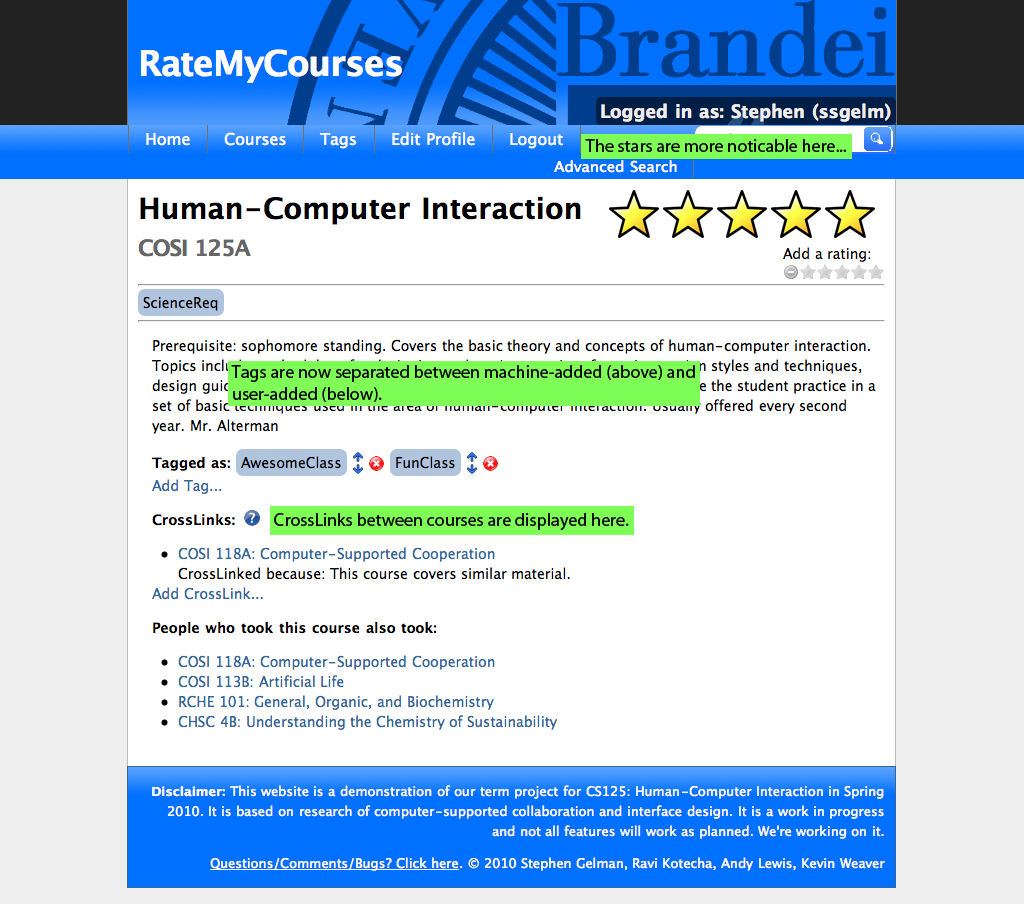
\includegraphics[width=\textwidth]{narrative-4.png}
\caption{Voting on a course}
\label{fig:vote}
\end{figure}

\section{Adding a Crosslink}

Crosslinks are added from the course page as well.  To add a Crosslink, the user clicks on ``Add Crosslink...''.  A dialog pops up as in Figure~\ref{fig:crosslink}. From the add Crosslink dialog, the user can begin typing the name of a course and it will autocomplete it.  In addition, the user must enter a description of the Crosslink so that it has meaning.

\begin{figure}
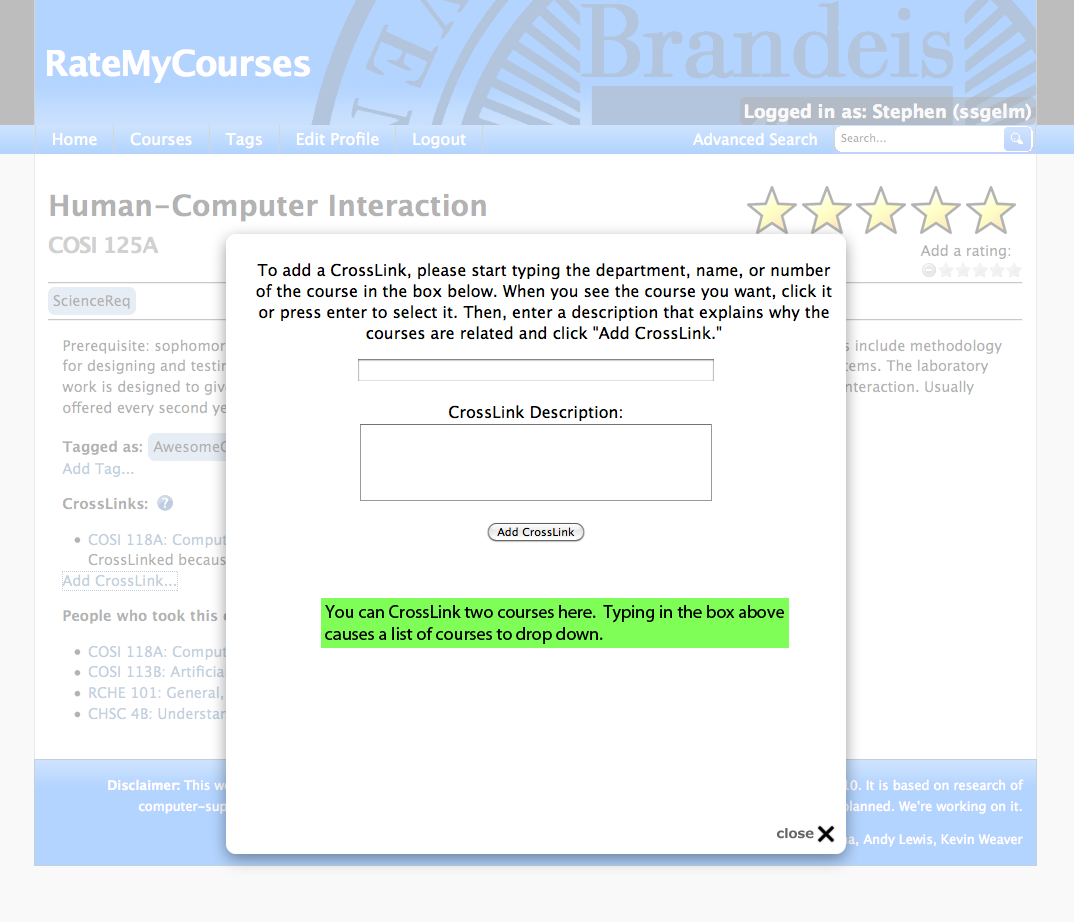
\includegraphics[width=\textwidth]{narrative-5.png}
\caption{Adding a Crosslink}
\label{fig:crosslink}
\end{figure}


\chapter{Analysis, Conclusion and Future Improvements}

\section{Analysis of Survey Data and Prototype Walkthroughs}

We designed a survey to distribute after the completion of prototype 2. We received 39 responses over the course of three days. Full survey response data can be found in the appendix. We began by asking general questions about their university status, class standing, and information on how they currently browse courses. From the data we gathered from Brandeis students, we can conclude that generally consult the Registrar's Course Catalog or the Student Union's Course Evaluation Guide a few times per year or semester, presumably around the course selection time. We then directed our questions specifically toward RateMyCourses. A majority of the participants reported that the overall purpose of the site was easily conveyed and for specific tasks such as finding, rating and tagging, the tasks were simple to complete.

The feedback we received from open-ended questions in the survey, as well as the prototype walkthroughs (also in the appendix), provide interesting suggestions, ideas and problems with our current design. Overall, user testing, interviews, GOMS and design heuristics evaluations, reveal that we still have a way to go in terms of error detection and prevention, help, documentation, features and usability. Users brought to our attention ideas and problems that we did not think about, thus highlighting the importance of having the end-user in the design process.


\section{Conclusion}

Overall, we made great progress since we began developing this project in Spring 2009 for CS118. Particularly between Prototypes 1 and 2 this semester, we focused on a few key features, implementing them the best we could, making sure to get feedback from end-users. The interface has become much cleaner and simplified. Aesthetically, we implemented a new CSS layout and completely re-worked the way users add tags (through an iFrame that pops up over the page) and browse the list of courses (tree view). We also added crosslinking and voting on tags, among other features. With Prototype 2 in production for only a few weeks, RateMyCourses holds the following statistics:

\begin{itemize}
\item 1891 courses in the database
\item 93 users (students and faculty)
\item 51 tags
\item 98 ratings
\item 8 Crosslinks
\end{itemize}

A majority of the users focused on the rating aspect of courses and a significant number added or created tags. Not many created crosslinks, either because they did not try or we did not clarify the meaning of this well enough.

We were constrained by time and resources throughout the development cycle. Though we spoke with plenty of students, we would have liked to have had time to speak with more professors, staff and administrators. As we learned this semester, design is an iterative process and it is not possible to create the best design in the first attempt. We still have many ideas and visions for RateMyCouses and have seen much improvement through each iteration.

\section{Future Improvements}

\subsection{Recommendation engine}

A major improvement to the RMC web application would be a recommendation engine similar to that of Netflix or Amazon.com.  The recommendation engine would be capable of giving each user a list of courses that they may find interesting.  Ideally, it would be based on courses that the user has previously rated or cross-linked.  The star rating system, tagged courses, and a way to save courses that have been rated would probably be important for this.

\subsection{A ``Locker'' for each user}

A ``Locker'' would allow each user to have a half-private/half-public profile page that included a list of courses they have taken, a list a courses they have bookmarked and wanted to save for later, and also a comments section. The comments section would allow users to get feedback from other users and potentially receive recommendations for each person.  Ideally, the recommendation engine would make this piece unnecessary, but computers make mistakes.

\subsection{Help Section}

It would be useful to have a documented help section that explains what things mean on the site, as well as a tutorial for new users.  The tutorial would have a simplified ``How-to'' that would explain how to add tags, add ratings, crosslink, etc.  We believe the interface is extremely intuitive, but this would still be helpful.


\appendix

\chapter{Prototype 1}

\section{Initial User Interviews}

\subsection{Script Outline}

\begin{enumerate}
\item What is your university affiliation?
\item If undergrad student, what is your class year?
\item What is your major(s) and minor(s)?
\item What are some important factors when deciding what classes to enroll in?
	\begin{enumerate}
    \item Please list factors in order of importance.
    \item How do you go about specifically choosing what courses to take, based on these factors?
    \end{enumerate}
\item How important is it to take classes out of interest rather than to fulfill a specific requirement?
\item How do you find courses related to your interests, but not in your major/minor?
\item How easy is it to find courses or information about courses from the current course guide on the Registrar's website?
\end{enumerate}

\subsection{Interview 1}

\begin{enumerate}
\item What is your university affiliation? \textbf{Student}
\item If undergrad student, what is your class year? \textbf{Senior}
\item What is your major(s) and minor(s)? \textbf{IIM: Communication and Media Studies, Minor in Business}
\item What are some important factors when deciding what classes to enroll in? \textbf{relevance to major, relevance to career path, schedule, professor, rating from course evaluation guide, workload rating}
	\begin{enumerate}
    \item Please list factors in order of importance. \textbf{relevance to career path, relevance to major, professor/rating from the course evaluation guide, schedule, workload rating}
    \item How do you go about specifically choosing what courses to take, based on these factors? \textbf{I pick my required courses first then I determine next courses based on what will work with the timing of the essential courses. Then I decide what courses look the most interesting that work with that schedule.}
    \item How do you decide what classes look the most interesting? \textbf{I look in departments that I find the most interesting or that I know I have a history of enjoying classes from those departments. Then I look for the most interesting title and read the summary, then review the course and professor rating.}
    \end{enumerate}
\item How important is it to take classes out of interest rather than to fulfill a specific requirement? \textbf{It’s very important because obviously you need to take the required courses, but being able to take classes that spark your interests is one of the greatest benefits of being a college student. It offers a unique experience that you won’t be able to get in the rest of your life.}
\item How easy is it to find courses or information about courses from the current course guide on the Registrar's website? \textbf{Information about courses could be more detailed in terms of the description. It might be too short of a description. I feel it could use another paragraph or two because it is often vague. The navigation of the overall Registrar’s site is good though.}
\end{enumerate}

\subsection{Interview 2}

\begin{enumerate}
\item What is your university affiliation? \textbf{Student, undergrad.}
\item If undergrad student, what is your class year? \textbf{Senior.}
\item What is your major(s) and minor(s)? \textbf{Politics and Economics, with a Legal Studies minor.}
\item What are some important factors when deciding what classes to enroll in? \textbf{Course time, professor, major/minor requirements, university requirements, interest.}
	\begin{enumerate}
    \item Please list factors in order of importance. \textbf{Time, major/minor requirements, university requirements, interest, professor.}
    \item How do you go about specifically choosing what courses to take, based on these factors? \textbf{Go through the schedule looking for courses to fill major/minor requirements, then search for ones with good times, then check description for interest, then check the professor.}
   	\item How often do you use the website each semester? \textbf{Check a few times during registration, then a few times during the add/drop period.}
    \end{enumerate}
\item How important is it to take classes out of interest rather than to fulfill a specific requirement? \textbf{It's important, if you take only required classes, that means you are not expanding your horizons, and it can get pretty boring. I've taken a few courses that fulfill no requirements because I needed to try something different.}
\item How do you find courses related to your interests, but not in your major/minor? \textbf{Word of mouth (recommendations from friends), and I know some of my general interests (e.g. chem, cosi).}
	\begin{enumerate}
	\item Is there useful info in registrar's site to find these courses? \textbf{No, because you cannot search based on the course description.}
	\end{enumerate}
\item How easy is it to find courses or information about courses from the current course guide on the Registrar's website? \textbf{Fairly easy, most difficult task is finding one more course based on interest (after filling schedule with required courses).}
\item Are there any changes to the registrar's site or CEG that you would like to see? \textbf{I would like to see scores for courses grouped by major (e.g. see how politics majors rated a chemistry course).}
\end{enumerate}

\subsection{Interview 3}

\begin{enumerate}
\item What is your university affiliation? \textbf{Student}
\item If undergrad student, what is your class year? \textbf{Junior}
\item What is your major(s) and minor(s)? \textbf{Studio Art and Classical Studies}
\item What are some important factors when deciding what classes to enroll in? \textbf{major requirements, interest level based on descriptions for classes in other departments, scheduling}
	\begin{enumerate}
    \item Please list factors in order of importance. \textbf{major requirements, interest level based on descriptions for classes in other departments, scheduling}
    \item How do you go about specifically choosing what courses to take, based on these factors? \textbf{majors - the two majors, then history, english pscychology what needs to be taken and then whatever works best}
    \end{enumerate}
\item How important is it to take classes out of interest rather than to fulfill a specific requirement? \textbf{the requirements have to be done but emphasis is placed on classes of interest as long as requirements are also being met}
\item How do you find courses related to your interests, but not in your major/minor? \textbf{just look through all of the majors, mostly humanities ones and read the titles/descriptions and also cross-listed courses from the taken majors}
\item How easy is it to find courses or information about courses from the current course guide on the Registrar's website? \textbf{it's easy to search based on requirements}
\item Would it be useful to search other departments more easily to find related courses? \textbf{Yes}
\item Friend recommendations? \textbf{Not that important, but could be a factor in deciding between two courses}
\item Are there any changes you would like to see to the registrars site? \textbf{See classes from other semesters, when the last time it was offered would be useful}
\item Are you familiar with the CEG on the Student Union website? \textbf{Wait they do that? Hmm I might have used it freshman year but I didn't think that it was that useful.}
\end{enumerate}

\subsection{Interview 4}

\begin{enumerate}
\item What is your university affiliation? \textbf{Student}
\item If undergrad student, what is your class year? \textbf{Senior}
\item What is your major(s) and minor(s)? \textbf{Chemistry, History (minor)}
\item What are some important factors when deciding what classes to enroll in? \textbf{requirements, interests}
	\begin{enumerate}
    \item Please list factors in order of importance. \textbf{requirements, interests}
    \item How do you go about specifically choosing what courses to take, based on these factors? \textbf{Look at the course list, start with Chemistry and go from there, department by department}
    \end{enumerate}
\item How important is it to take classes out of interest rather than to fulfill a specific requirement? \textbf{brings excitement into life, requirements are prioritized}
\item How do you find courses related to your interests, but not in your major/minor? \textbf{Start looking through departments based on opening in the schedule, perhaps use the search by time}
\item How easy is it to find courses or information about courses from the current course guide on the Registrar's website? \textbf{it's fine}
\item Would it be useful to search other departments more easily to find related courses? \textbf{Yes. ``if you like this, you might also like''}
\item Friend recommendations? \textbf{Depends on the friend}
\item Are there any changes you would like to see to the registrars site? \textbf{No.}
\item Are you familiar with the CEG on the Student Union website? \textbf{Yes, doesn't use it because he is lazy}
\end{enumerate}

\section{Cognitive Walkthrough}

\subsection{Task 1: Navigating to an individual course page}

\begin{enumerate}
\item Define Inputs to the walkthrough
	\begin{enumerate}
    \item Identification of the users
    	\begin{enumerate}
        \item Students and faculty at Brandeis 
        \end{enumerate}
    \item Action sequences for completing the task
    	\begin{enumerate}
        \item Click ``Login''
        \item Then click ``courses''
       	\item Either find a class by using the page numbers or select a department from the drop down menu.
        \item Click the link for the desired course.
        \end{enumerate}
 --OR-- 
        \begin{enumerate}
        \item Click ``Login''
        \item Then type in a search query in the search box
        \item Press enter to search.
        \item Click on the desired search result. 
        \end{enumerate}
    \item Description of implementation of the interface
        \begin{enumerate}
        \item Users can find a class by either browsing the course listing, or by searching by keywords. 
        \end{enumerate}
	\end{enumerate}
\item Convene the analysts
\item Walk through the action sequences for each task
	\begin{enumerate}
    \item Tell a credible story, considering
    	\begin{enumerate}
        \item Will the user try to achieve right effect?
        	\begin{enumerate}
            \item The naming convention should make it clear that a course can be found by clicking the courses button or by searching. It is assumed that a user will know that they have to find a course in order to view a description, add a tag, or do any other function related to finding the course.
            \end{enumerate}
        \item Will the user notice that the correct action is available?
            \begin{enumerate}
            \item If the user wants to find a course, they obvious link is the one that says ``Courses.'' However, when they search for one, they might not realize that they can pick by department rather than by going through each page. An issue is that the pages are random. The user may not be able to easily find the right page to find the course they want, which could be frustrating. 
            \end{enumerate}
        \item Will the user associate the correct action with the effect that user is trying to achieve?
            \begin{enumerate}
            \item If the search string does not match any course names, the search will yield minimal results, if any. Since ``Courses'' lists a manifest of all the available courses, it is likely the user will understand what will happen if they click that button.
            \end{enumerate}
        \item If the correct action is performed, will the user see that progress is being made toward solution to the task?
            \begin{enumerate}
            \item After any link is clicked, another page opens. If they open the course page, they will see the information for that particular course.
            \end{enumerate}
    	\end{enumerate}
	\end{enumerate}
\item Record Critical Information
	\begin{enumerate}
    \item User knowledge requirements
    	\begin{enumerate}
    	\item The user needs to know what courses exist and perhaps their departments if they try to browse by name.
        \item The user has to understand why they want to find a course. 
       	\end{enumerate}
    \item Assumptions about the user population
        \begin{enumerate}
    	\item We are assuming people know what departments the classes they have taken are in and that the users go to Brandeis. The website requires a Brandeis user name and password, so we assume they are members of the Brandeis community with a valid login.
        \item We assume people can get to the website.
        \end{enumerate}
    \item Notes about side issues and design changes
        \begin{enumerate}
    	\item Users may not know what they can search for or how to actually find a course without trial and error.
        \item A description or some kind of text needs to be added to the front page to inform users what their possible actions are and a help section to tell them how to do it and why. 
        \end{enumerate}
	\end{enumerate}
\end{enumerate}

\subsection{Task 2: Add a tag}

\begin{enumerate}
\item Define Inputs to the walkthrough
	\begin{enumerate}
    \item Identification of the users
    	\begin{enumerate}
        \item Students and faculty at Brandeis 
        \end{enumerate}
    \item Action sequences for completing the task
    	\begin{enumerate}
        \item Follow steps in Task 1 to find a course and then click on it to open the page for that specific course
        \item Read the tags listed underneath the description of the course to decide if a tag needs to be added
        \item To add a tag, click on the drop down menu to select an existing tag, or click “Add new tag” at the bottom of the drop-down. o iv. Type in the tag in camel case.
        \item Click ‘OK’
        \end{enumerate}
    \item Description of implementation of the interface
    	\begin{enumerate}
        \item Users will go to the website, and then after logging in, try to find a course and they may decide to tag it. Tagging allows for a way to describe attributes of a particular course and a tag can be shared by multiple courses, which in a way, relates them.
        \end{enumerate}
    \end{enumerate}
\item Convene the analysts
\item Walk through the action sequences for each task
	\begin{enumerate}
    \item Tell a credible story, considering
    	\begin{enumerate}
        \item Will the user try to achieve right effect?
        	\begin{enumerate}
            \item The user may not actually know what the purpose of tagging is and if they select the wrong tag, there’s no easy way for the user to delete the tag they just added. 
          	\end{enumerate}
        \item Will the user notice that the correct action is available?
            \begin{enumerate}
            \item The drop down menu right below the list of existing tags says “Add a tag.”
            \item They may not realize that there is a drop down and may think they have to click a link and will see another page to actually select the tag they want.
            \item They may also think that “Add a tag” means to type in their own tag. 
            \end{enumerate}
        \item Will the user associate the correct action with the effect that user is trying to achieve?
            \begin{enumerate}
            \item There is a possibility that the user will not know how to add a description to a course. There isn’t a definition of what tags are and what they can be. This could cause confusion to a beginner. 
            \end{enumerate}
        \item If the correct action is performed, will the user see that progress is being made toward solution to the task?
            \begin{enumerate}
            \item After the tag is added, it will appear on the course page. 
            \end{enumerate}
      	\end{enumerate}
   \end{enumerate}
\item Record Critical Information
	\begin{enumerate}
    \item User knowledge requirements
    	\begin{enumerate}
        \item The user needs to know how to find courses
        \item The user needs to know what the purpose of a tag is and why they want to add one. 
        \end{enumerate}
    \item Assumptions about the user population
        \begin{enumerate}
        \item We are assuming people know what departments the classes they have taken are in and that the users go to Brandeis. The website requires a Brandeis user name and password.
        \item We assume people can get to the website. 
        \end{enumerate}
    \item Notes about side issues and design changes
        \begin{enumerate}
        \item  Make it obvious that the user needs to login before they can tag courses.
        \item Change the design of how to add a tag to a course. The conceptual model is not clear. The tags may also need to be categorized so system tags do not appear. 
        \end{enumerate}
    \end{enumerate}
\end{enumerate}


\section{Screenshots}

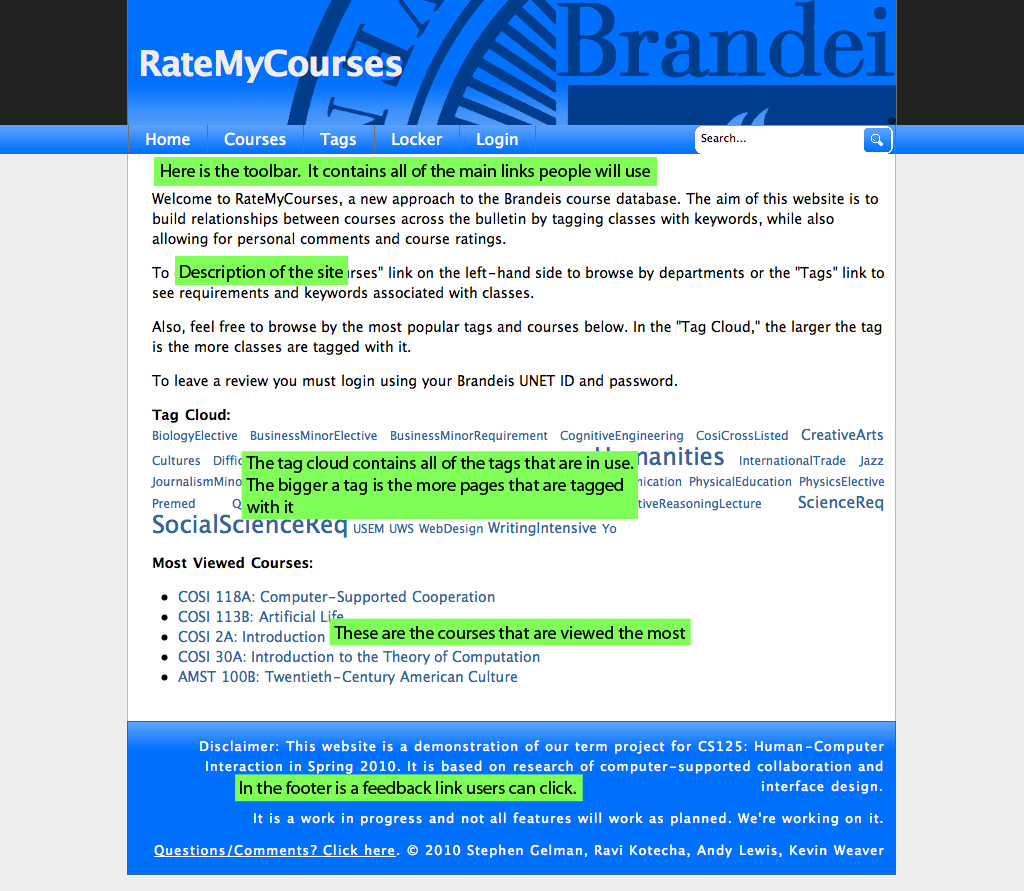
\includegraphics[width=\textwidth]{screen-1.png}
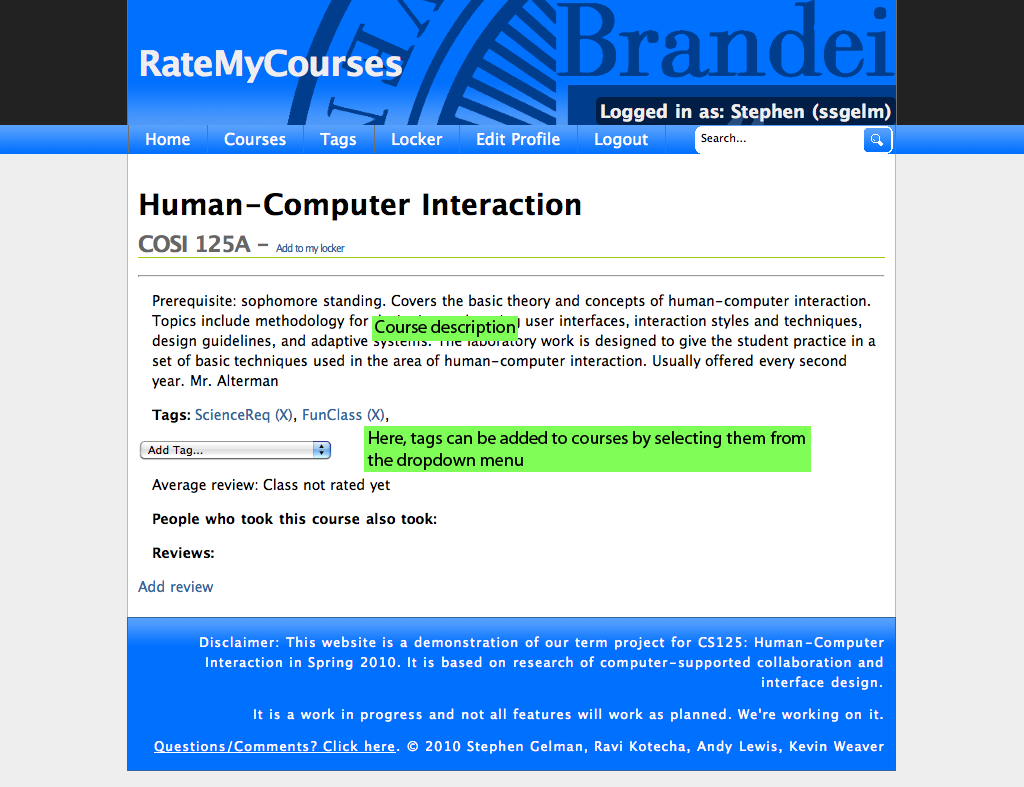
\includegraphics[width=\textwidth]{screen-2.png}
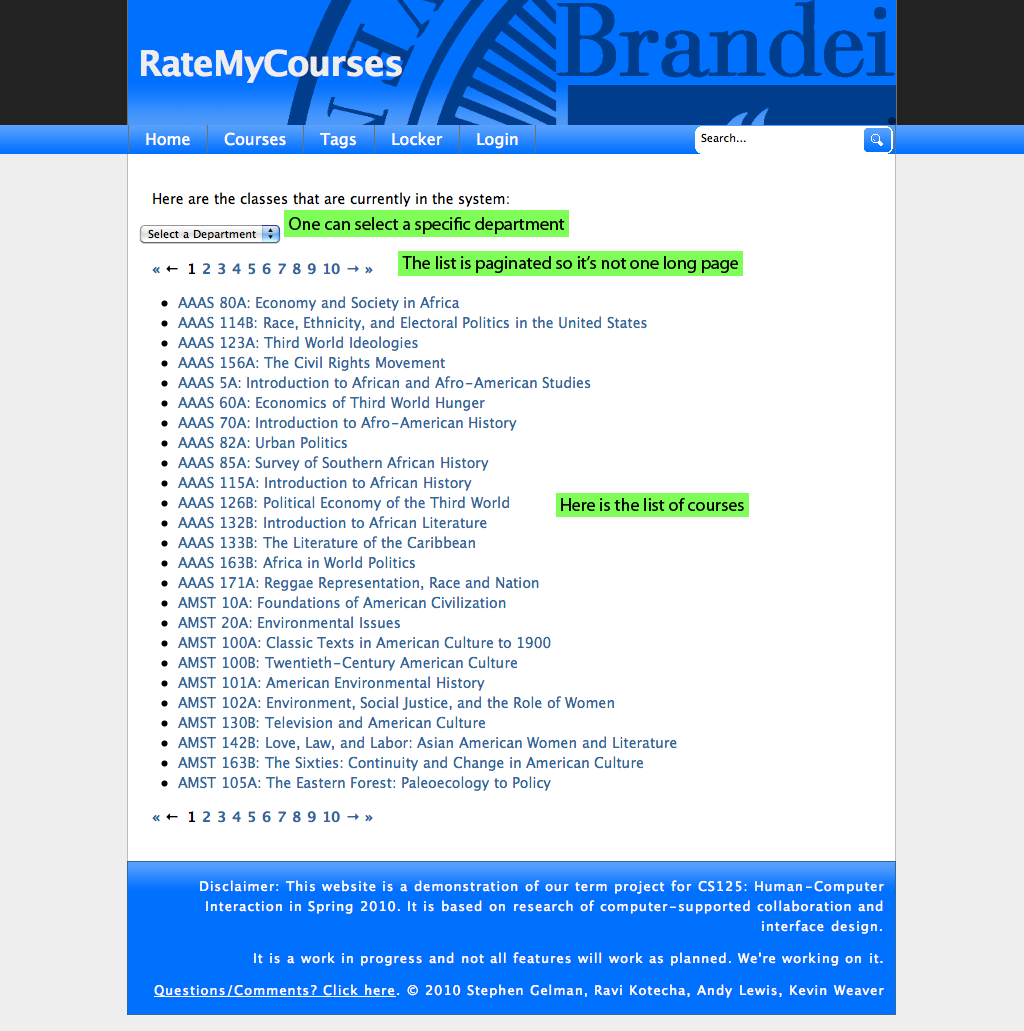
\includegraphics[width=\textwidth]{screen-3.png}
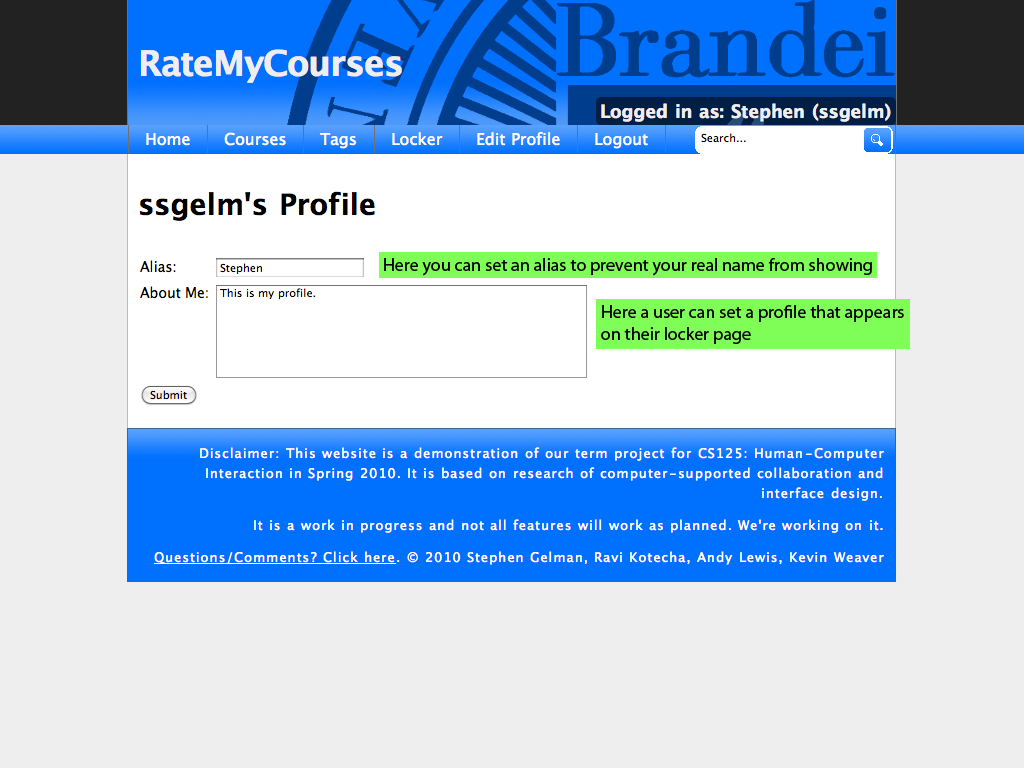
\includegraphics[width=\textwidth]{screen-4.png}
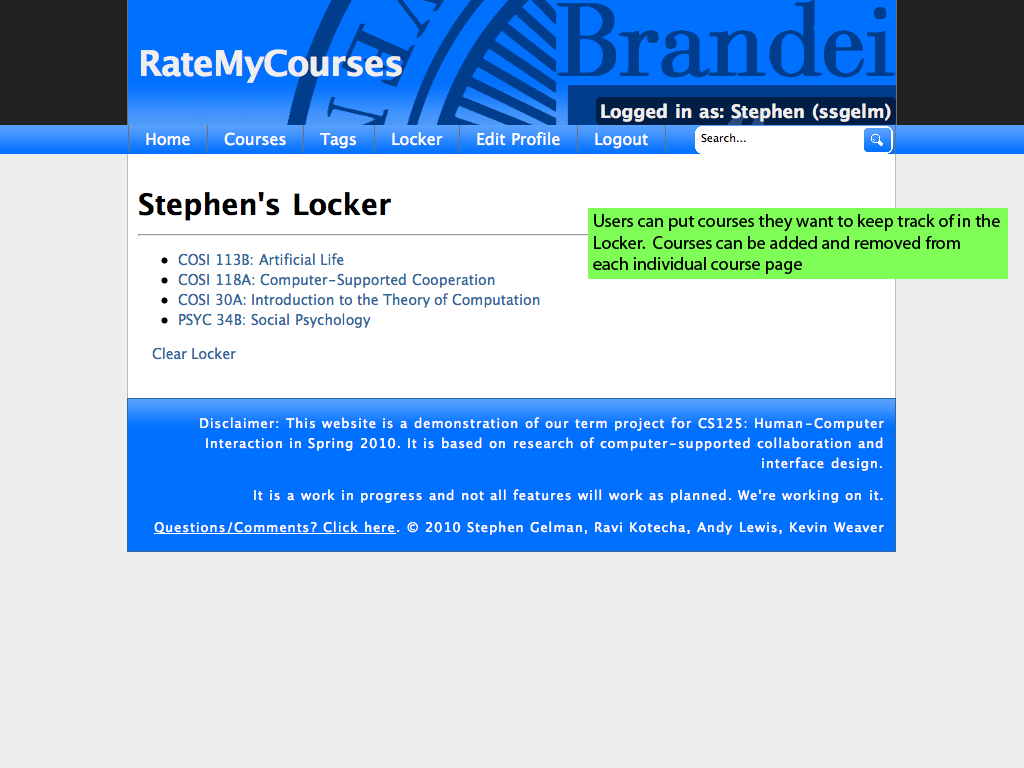
\includegraphics[width=\textwidth]{screen-5.png}
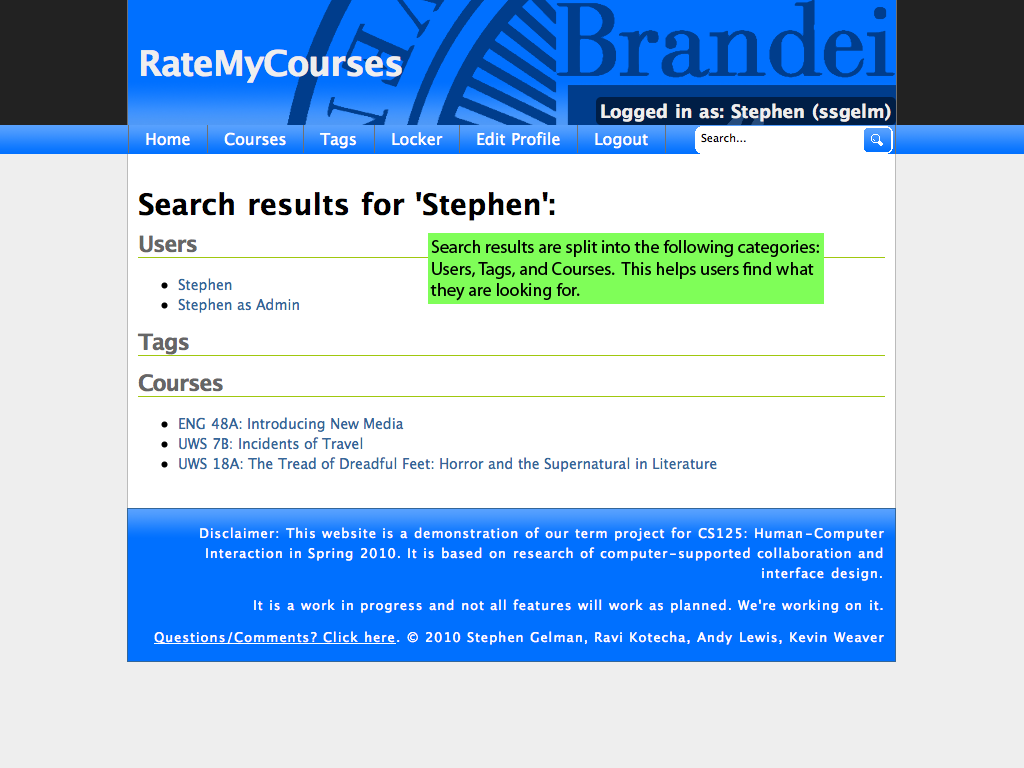
\includegraphics[width=\textwidth]{screen-6.png}
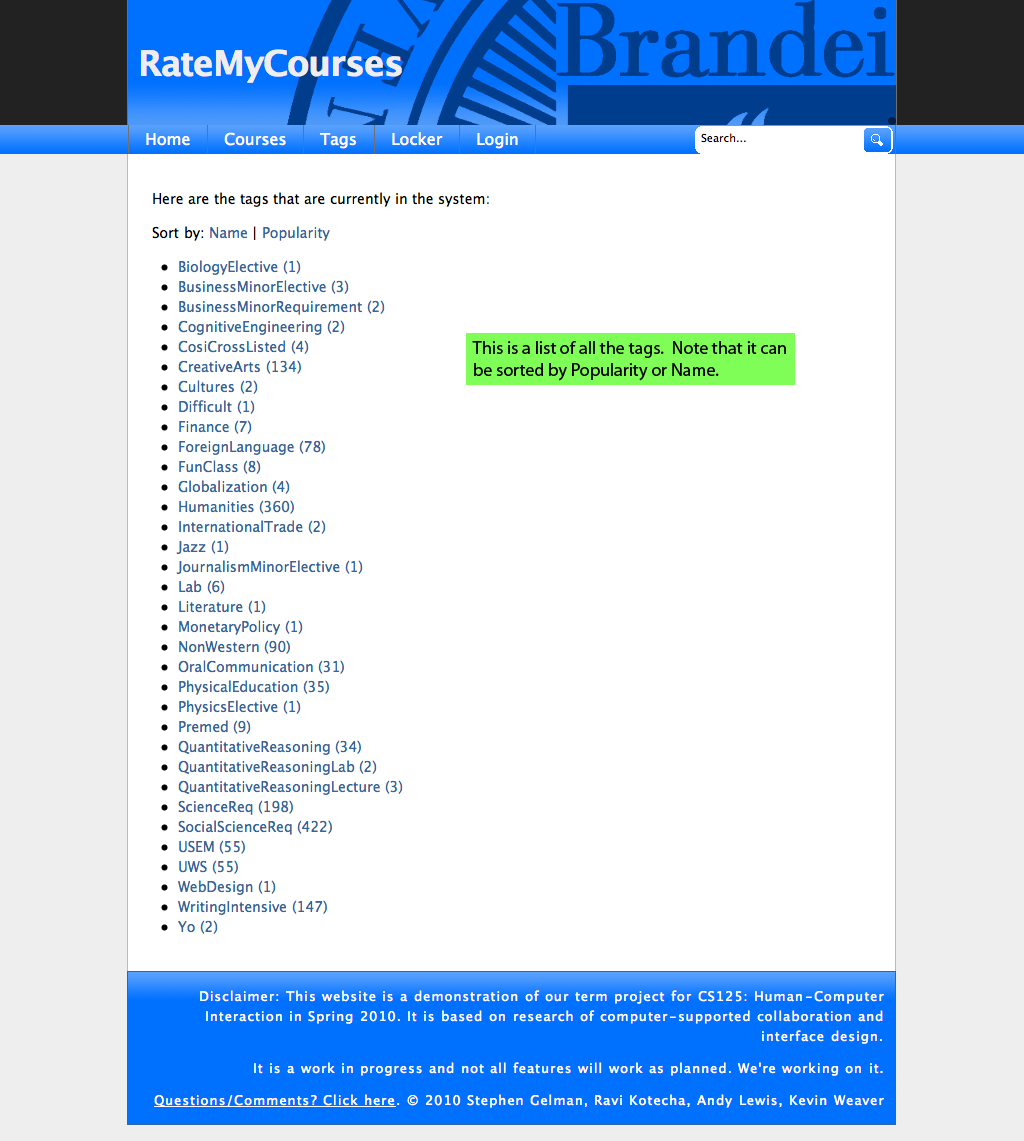
\includegraphics[width=\textwidth]{screen-7.png}

\section{Walkthrough Comments}

\subsection{Walkthrough 1}

\begin{itemize}
\item Likes design, no big paragraphs
\item Good searching
	\begin{itemize}
    \item Would use search box
    \item Usage: would type course number if looking for specific course otherwise, would browse using ``Courses'' tab 
    \end{itemize}
\item Consistent with Registar's site (dropdown box)
\item page layout: questions order of courses (not in numerical order by course number, should be consistent)
\item Course pagination make sense with arrows, but unlikely that someone would browse that far
\item Dropdown menu does not work at the moment look at COSI 11a
\item Likes our importation of Registar's description and requirements
\item Figured out usefulness of tags quickly
\item Likes ``people who took this also liked...''
\item Adding a tag to a course
\item Searched for ``ECON 2a'' and did not find course, searched for ``ECON'' and found it
\item Likes ``do you find this review useful/inappropriate''
\item Tried to add tag, needed to log in, but Cosign authentication redirected back to home page
\item Added ``Fun Class''

\item Questioned allowing everyone to add tags
    \begin{itemize}
    \item Moderator would be most useful for inappropriate tag, but that could be a full-time job
    \item Next best way would be ``is this tag inappropriate?'' button with reason - I mentioned voting, he thought it would be useful 
    \end{itemize}

\item Incentive to rate courses: prizes?
\end{itemize}

\subsection{Walkthrough 2}

Home Page:
\begin{itemize}
\item Tag cloud: stands out and very useful. Really shows what kind of information people are looking for. It's a really interesting concept. Very informative visually.
\item Nice and simple layout
\item Not too many options
\item User friendly 
\end{itemize}
Looking for a class:
\begin{itemize}
\item Page numbers make it difficult to figure out what letters in the alphabet fall on each page
\item Suggestion: change the numbers to letters
\item Four-letter codes for departments are not always clear, suggests display whole name of department next to 4 letter code Individual class page:
\item Tags seem appropriate
\item Consistent course description
\item Add Tag vs. New Tag labels in tag list not clear or intuitive
\item Created new tag
\item Tried to put a space in the tag name caused an error ``Handling bad tags:''
\item Should be handled by the Registrar 
\end{itemize}
Overall:
\begin{itemize}
\item Just as useful as the course evaluation guide
\item Impressed
\end{itemize}

\subsection{Walkthrough 3}

Home Page:
\begin{itemize}
\item Meaning of tag cloud not clear
\item Layout easy to read, follows Brandeis color scheme of blue and white
\item Simple Course Listing: 
	\begin{itemize}
    \item Alphabetical listing by course load 
	\end{itemize}
\item Arrows navigating page numbers not clear
\item Department listing needs indication of what the four letters stand for 
\end{itemize}
Course Page:
\begin{itemize}
\item Easy to read
\item Clearly marked and labeled 
\item Course description consistent with Registrar 
\end{itemize}
Adding a tag:
\begin{itemize}
\item Tag listing relatively makes sense. Some definitions are not clear.
\item User added a new tag
\item Enter Tag dialog box not clear about spacing, capitalization, consistency of tag names
\item After login, does not return user to current page. Instead he has to re-navigate to where he was and re-add the tag again.
\end{itemize}


\chapter{Prototype 2}

\section{Expert Reviews}

\subsection{Nielsen’s Ten Usability Heuristics}

\begin{description}
\item[Visibility of System Status] RMC Prototype 2 is designed to ensure the visibility of the system status. At any page, the header displays whether or not a user is logged in, and if so says “Logged in as: …”. Additionally, green or red status menus appear throughout the site based on response to user action. For example, after logging in, the system displays a green box saying: “You are now logged in as alewis1!” Additional menus to ensure visibility of status appear after tagging, searching, and adding crosslinks.
\item[Match between System and the Real World] The language used throughout the site is simple, clear and easy to understand. Between prototypes, we made sure to remove technical terms in headers, menus and bodies of individual pages and replace them with non-technical equivalents. For example, “course database” was changed to “course catalog”, which reflects the language of the end-user (students, faculty and staff) rather than our individual technical backgrounds. We worked with a student majoring in Media and Communications to help re-write the text across the site.
\item[User control and freedom] Since this is a website, a large part of user control and freedom is controlled via the user’s web browser, using the back and forward buttons to navigate between their browsing history. Tabs on the header of each page provide a clear way to navigate between the different pages of the site. However, there lacks an “undo” or “redo” feature when adding tags, crosslinks, or ratings. There is no way to undo an action here, and any error or mistake must be corrected from the back-end by an RMC administrator.
\item[Consistency and Standards] The layout of this prototype follows the conventions of most websites and is easy to navigate.  Overall the site uses consistent language with that of the Registrar and Student Union Course Evaluation sites.
\item[Error Prevention] RMC provides good error messages only in certain cases. In entering an invalid search term or rating a class one previously rated, the system provides good feedback to the user that the current action is not possible. However, in the case of adding an incorrect or misspelled tag or crosslink listing, after hitting “Submit” there is no way to re-confirm or undo an action. For example, if I misspell a tag, the only way to get rid of it is to delete it from the back-end database.
\item[Recognition over Recall] Performing tasks in RMC relies on recognition rather than recall. In using the system, the user does not have to remember or recall anything. In the courses tab, RMC displays all of the Brandeis courses, categorized by department. In adding a tag, RMC displays all of the tags in the system and a user can choose from the list. In adding a crosslink, the RMC engine auto-completes based on the user’s input.
\item[Flexibility and Efficiency of Use] We included a few “accelerators” to enhance the use of the system for advanced users, such as the ability to do an advanced search based on multiple tags. Also, when tagging a course, the auto-complete textbox allows advanced users to directly enter a tag name rather than search through the whole list of tags.
\item[Aesthetic and Minimalist Design] This site has a simple and minimal CSS layout and overall site design. Sections of an individual page are separated through color, using blue for the header and footer and white for the body. Tags have a distinct look, with black text and a grey background.
\item [Error Recovery] Overall, errors and messages are clearly expressed in plain language. Error messages pop up as a red background, while success messages have a green background. The error messages clearly detect and help users recognize errors, however the error dialogues do not always provide clear information on how to recover from the error.
\item[Help and Documentation] Though not yet fully implemented, RMC provides help and documentation to the user.  On the home page, we provide three scenarios for users to start using RMC: 1) a walkthrough of the site, 2) login, and 3) just browse the site without logging in. Also, individual pages for tags provide a space for tag definition. An example can be seen here: https://ratemycourses.brandeis.edu/tag/Premed. Additionally, there is a quick help feature for the Crosslink function. On any individual course page, a question mark appears next to Crosslink, which is a tooltip that explains the definition of Crosslink.
\end{description}


\subsection{Shneiderman’s Eight Golden Rules of Interface Design}

\begin{description}
\item[Consistency] RMC holds a consistent interface throughout the website. Aesthetically, the site uses the same fonts, layout, color and styles throughout each page. The language used is consistent across pages, as well as consistent with the language on the Registrar and Course Evaluation Guide websites.
\item[User Shortcuts] Though not yet implemented, through the Home Page RMC can provide a tutorial or walkthrough for beginning users, giving them a demonstration of what the website is about and how to use it. Expert users can simply begin using the site right away. Explanations, through text or tooltips, describe or simplify tasks. We implemented large fonts throughout the site and clean, simple layouts. Overall RMC is well designed to cater to all levels of users.
\item[Feedback] Feedback involving interaction with tasks is generally provided through dialog boxes (both success and error messages). Tagging, searching and crosslinking all offer informative feedback as to state of the system. Since this is a website, feedback when interacting with an individual page is provided through mouse-over actions, such as highlighting, changing the background color of the hyperlink, or fade effects.
\item[Design Dialogs to Yield Closure] Dialogs, and tasks, are designed to yield closure. For example, when adding a tag, the beginning sequence is clicking the “Add Tag” link, the middle sequence is the iframe which displays the dialog box to add a tag, and the end sequence is clicking submit, which displays a dialog box indicating success or failure of the task. Also, on the Courses page, the tree-view list of courses is designed to yield closure, in this case the selection of an individual course.
\item[Error Prevention and Handling] RMC does not fully prevent errors. There is no error checking when adding a tag, and for example I can enter random digits, which becomes a tag. In this case, or in the case of misspelled or incorrectly chosen tag, there is no confirmation to ensure correctness or no way to undo this action. These errors have a cascading effect. One incorrect or misspelled tag created by one user turns into an option for the next user.
\item[Easy Reversal of Actions] Reversal of actions is easy if users navigate to a specific page by mistake. This can be reversed by using the browser’s back and forward navigation buttons, as well as by clicking the appropriate tab in the header (which appears on each page).
\item[Internal Locus of Control] Overall RMC does a good job of supporting internal locus of control. Good feedback ensures that users feel that the interface responds to their actions.  Interface interactions are designed to be as simple as possible, and any one task involves a short sequence of actions. Information is clearly displayed throughout the site. When adding tags or crosslinks, RMC is designed to minimize the amount of tedious data entry necessary. When adding tags, the iframe lists all the tags in the system at once, or textbox to enter a tag autocompletes using the results in the system. When adding a crosslink, the search box autocompletes using the courses in the system. Overall, all of these features, as well as others, help users feel like they are in control of the interface.
\item[Reduce Short-term Memory Load] The RMC interface is designed to reduce short-term memory load, though it could use more work with this. When adding a tag, the list of tags does not display their corresponding definitions, which requires users to remember the definition. Generally, the definitions are obvious, however in some cases there may be semantic differences in the tag meaning.
\end{description}

\subsection{Donald Norman’s Usability Principles}

\begin{description}
\item[Visibility] Actions possible by RMC are clear and visible on each page. In the header of each page contains links to each section: the home page, list of all courses, list of all tags, login, and basic and advanced searches. On the all courses page, the tree view makes visible a lot of information at once; it lists each academic department at Brandeis, and once expanded, each course within that department. The layout of the individual course page visibly displays all possible actions: add a rating, tag a class, and select a crosslink.
\item[Feedback] Overall the site provides good feedback through the use of mouse-over actions and dialog boxes.
\item[Constraints] Tasks on RMC are designed with artificial constraints. For example, the tasks of rating, tagging or crosslinking are only possible once a user has authenticated via their Brandeis Unet ID. We reduced the need for knowledge, and have users rely on recall through icons and visuals. Ratings, for example, are visually displayed in terms of stars. Through the use of color, tags are displayed as icons.
\item[Mapping] Through the use of icons, hyperlinks and text, there exists mappings between intentions and possible actions. Additionally, through immediate feedback from actions, users can always determine the system state. Overall, the system responds to user intentions.
\item[Affordance] RMC contains good affordances that take advantage of web conventions, such as clicking on hyperlinks and pushing buttons to submit a form.
\item[Good Conceptual Model] Overall, RateMyCourses has a good conceptual model. Because of the heavy use of tagging in Facebook, most college students are already familiar with the concept of tagging. We took this familiar concept and applied it to the Registrar’s Bulletin. Though RMC is still in its initial stages and has a very small amount of usage data, it has the potential to become a vital tool in the exploration of classes across departments.
\end{description}

\section{GOMS analysis}


Key:
\begin{description}
\item[K] type a key
\item[P] point to a position on screen
\item[H] homing
\item[M] mentally preparing for next step
\item[R] responding
\item[L] login through Brandeis' Cosign system
\end{description}
Logging in through Cosign (http://login.brandeis.edu)
\begin{itemize}
\item P H Kx H M Ky K
    \begin{itemize}
    \item x is the number of letters in the username
    \item y is the number of letters in a password 
    \end{itemize}
\end{itemize}
Finding a course
\begin{itemize}
\item Click courses tab with mouse
\item Read and evaluate the tree-view of courses
\item Click on department name
\item Click on course
\item P M P P
\end{itemize}
Tagging a course
\begin{itemize}
\item Find the course
\item Click “add tag”
    \begin{itemize}
    \item New tag
    \item Type in name of tag
    \item Click ``Add Tag''
    \item Existing tag
          \begin{itemize}
          \item Find tag in tag cloud
          \item Click tag
          \end{itemize}
    \end{itemize}
\item New tag:
    \begin{itemize}
    \item P M P P M P H Kx H P
    \item Where x is the number of letters in the tag
    \end{itemize}
\item Existing tag:
    \begin{itemize}
    \item P M P P P
    \end{itemize}
\end{itemize}
Crosslink
\begin{itemize}
\item Find a course
\item Click Crosslink
\item Move mouse to course field
\item Begin typing course name
\item Select course from list with mouse
\item Click on description field
\item Type in description 
\item P M P P P M P H Kx H P P M Kx
\end{itemize}
Rating
\begin{itemize}
\item Find a course
\item Click on star value to add rating
\item P M P P M P
\end{itemize}

\section{Walkthrough Comments}

\subsection{Walkthrough 1}
Home page

\begin{itemize}
\item Background shading for tags is good because it gives better separation
\item ``New to RateMyCourses'' box gives better information on how to use the site
\end{itemize}
Courses Listing
\begin{itemize}
\item Tree view display of classes does not display in Internet Explorer
\item User found course through Search box
\end{itemize}
Individual Course Page
\begin{itemize}
\item Likes the fact that the requirements are up top right below the title, that is one of the most important factors people look at when choosing classes
\item ``Course not rated yet'' is good because it gives the system state, in that it is not rated
\item Tooltip to explain crosslinking is useful in helping define what exactly crosslinking is, as it is a confusing term
\item ``People who took this course also took'' is empty, which is misleading. Make it clear the way the recommendation engine works. This is confusing.
\end{itemize}
Rating a course
\begin{itemize}
\item ``Cool!''
\item A lag between selecting stars and the results appearing
\item Enjoys the green dialog box which explains that the action was completed successfully
\end{itemize}
Adding a tag
\begin{itemize}
\item iFrame does not work in Internet Explorer, redirects to new page
\item Directions clear
\item Adding a tag with spaces causes site to crash
\item Speculates that arrows cycle through tags. Explained real purpose, but participant said the arrows are not clear. Suggests adding tooltip.
\item User added a description for the tag to help other users.
\end{itemize}
Crosslinking
\begin{itemize}
\item Likes the auto-suggestion
\item Finds the interface intuitive
\item Text of ``Crosslink Description'' not immediately clear
\end{itemize}
Overall
\begin{itemize}
\item Overall much better than the current rating system
\item A few bugs, but once these are fixed Brandeis should use this instead
\end{itemize}

\subsection{Walkthrough 2}
  Home page:
\begin{itemize}
\item Why are some of these tags bigger?
\item What is the point of the tags?
\end{itemize}
  Course page
\begin{itemize}
\item No problems with this
\item What is the point of a Crosslink?
\item Adding a tag is simple and easy to use
\end{itemize}
General comments:
\begin{itemize}
\item Not easy to understand what is meant by a tag or why they are useful
\item Why are they called tags and not categories?
\item Probably wouldn't use this site
\end{itemize}

\subsection{Walkthrough 3}
Home page:
\begin{itemize}
\item ``Wow look at all the things I can click on''
\item A bit confusing at first
\item Liked ``new user'' option
\item Instinctively used tag cloud to find courses
\item Looked for tags that pertained to her, then her major, then a class she liked
\end{itemize}
Class page:
\begin{itemize}
\item First instinct is to rate
\item ``Can I write something?''
\item Liked the ``People who took...'' courses at the bottom
\item Enjoyed rating classes taken
\item Liked that requirements were listed for courses
\item Thought hovering over question mark was not obvious for Crosslink description
\item Wished it was possible to give half star ratings, i.e. 4.5/5 stars.
\item Liked feedback on rating
\item Wanted to be able to write reviews to understand particular ratings
\item More likely to rate a course because it was good than because it was bad
\item Would be helpful to know how many people had rated the course
\end{itemize}
Courses list:
\begin{itemize}
\item Found tree view intuitive
\item Located a course very quickly
\end{itemize}
Add tag:
\begin{itemize}
\item Tagging really cool idea
\item Liked potential for different tags
\item Instinct was to use existing tag instead of creating one
\end{itemize}
Tags:
\begin{itemize}
\item Liked to browse for course by tag: ``Let's see what classes were tagged with HotProfessor''
\end{itemize}
Crosslinking:
\begin{itemize}
\item Didn't understand the benefit at first, but once explained liked the idea
\end{itemize}
Search:
\begin{itemize}
\item ``That was really fast''
\item Not immediately obvious that search box exists
\item More likely to want to browse
\item Wanted to search by course number but it didn't work
\end{itemize}

\section{QUIS Survey Data}

We received 39 responses given over the course of three days. We designed this survey with a combination of drop-down, open-ended and Likert scale questions.

\subsection*{What is your university affiliation?}

\begin{tabular}{lll}
Response	&Percent Response	&Count \\
\hline
First-year student	&10.3	&4\\
Sophomore student	&25.6	&10\\
Junior student	&17.9	&7\\
Senior student	&46.2	&18\\
Graduate student	&0.0	&0\\
Faculty	&0.0	&0\\
Staff	&0.0	&0\\
\end{tabular}

\subsection*{How frequently do you find yourself browsing the course catalog?}

\begin{tabular}{p{8cm}ll}
Response	&Percent Response	&Count \\
\hline
Never	&2.6	&1\\
A few times each semester	&44.7	&17\\
Many times during one or two months out of the year	&42.1	&16\\
A few times each month on a regular basis	&10.5	&4\\
Every week	&0.0	&0\\
I didn't know this existed	&0.0	&0\\
Skipped question	&-	&1\\
\end{tabular}

\subsection*{How frequently do you find yourself browsing the Course Evaluation Guide?}

\begin{tabular}{p{8cm}ll}
Response	&Percent Response	&Count \\
\hline
Never	&28.9	&11\\
A few times each semester	&44.7	&17\\
Many times during one or two months out of the 	year	&21.1	&8\\
A few times each month on a regular basis	&2.6	&1\\
Every week	&0.0	&0\\
I didn't know this existed	&2.6	&1\\
Skipped question	&-	&1\\
\end{tabular}

\subsection*{After browsing RateMyCourses, how well do you feel you understand the purpose of the site?}

\resizebox{15cm}{!} {
\begin{tabular}{llllllll}
not at all	&somewhat well	&fairly well	&very well	&fully	&No Opinion	&Rating Average	&Response Count\\
\hline
5.6 (2)	&2.8 (1)	&27.8 (10)	&25.0 (9)	&38.9 (14)	&0.0 (0)	&3.89	&36\\
\end{tabular}
}

\subsection*{Please rate how easy you found it to complete the following tasks:}

\resizebox{15cm}{!} {
\begin{tabular}{lllllllll}
	&1	&2	&3	&4	&5	&6	&Rating Average	&Response Count\\
\hline
Finding a course	&0.0 (0)	&0.0 (0)	&0.0 (0)	&24.3 (9)	&75.7 (28)	&0.0 (0)	&4.76	&37\\
Rating a course	&2.7 (1)	&0.0 (0)	&2.7 (1)	&16.2 (6)	&59.5 (22)	&18.9 (7)	&4.60	&37\\
Tagging a course	&2.7 (1)	&0.0 (0)	&0.0 (0)	&13.5 (5)	&54.1 (20)	&29.7 (11)	&4.65	&37\\
Cross-linking two courses	&10.8 (4)	&0.0 (0)	&0.0 (0)	&21.6 (8)	&18.9 (7)	&48.6 (18)	&3.74	&37\\
\end{tabular}
}

\begin{enumerate}
\item I didn't know this was possible
\item Impossible
\item Difficult (required some help)
\item Easy (figured it out after some time)
\item Simple
\item I didn't try
\end{enumerate}

\subsection*{Was there anything you found to be particularly confusing?}

\begin{itemize}
\item When you search for classes using the advanced search, it seems like they come up in any random order (not in order). Also, when I searched the term ``real estate'' some classes came up more than once.
\item There should be a login button on the home page in one of the top corners in addition to ``I've been here before, log me in!'' since most people assume that there will be a login link in one of the top corners.
\item No.
\item There should be more directions
\item The purpose of this site
\item Perfectly clear all around
\item It wasn't initially clear that you could search by department. The homepage has all the funny boxes for various requirements that are fulfilled by a course, but the folder tabs by major were awesome
\item I believe the rating should be centered on the page instead of in the corner. As is, it looks more like just a course catalog instead of a rating system.
\item No
\item Really easy to navigate. Nice work guys.
\item No, great site!
\end{itemize}

\subsection*{Are there any features that you wish RateMyCourses had that would make it easier to use?}

\begin{itemize}
\item It would be better if once you rated a course, you could change the rating. When I tried to change the rating, it gave me an error message saying ``Course already rated.''
\item You couldn't untag something that you added accidentally
\item I would not user RateMyCourses in its current state. Every time a course is taught, it is taught completely differently. In fact, the most important variable in whether a course will be worth taking is the professor, not the course itself. In effect, all of these ratings will suffer from severe missing variable bias. The Course Evaluation Guide allows me to search both by professor and by course, and allows me to look up ratings of one specific offering of a course, which is much more useful to me.

Additionally, I find the tagging feature to be completely useless. Tagging depends on someone moderating to make sure that tags are consistently applied and that duplicate tags with similar spellings are not made. The most important tags, such as what requirements the course fulfills, can already be easily searched for on the Registrar's site.
\item No.
\item Perhaps if the courses were further broken down into sections. (Sometimes different teachers teach multiple sections of the same subject.)
\item A comments section might be nice. It would probably be more trouble than its worth, but getting more detailed opinions of a class would be helpful.
\item There should be an easily accessible list of the best and worst courses.

Optimally, there should be a way to rate different components of a course and then rank courses by their average scores for each category.
\item List of courses by department
\item A back button that will return you to the course tree with it expanded to how it was last. A comment section for each page that is not automatically displayed.
\item Rate Professors too???
\item No
\item Include more about professors
\item It should show the number of people who voted on a particular course.
\item I wish there was a way to comment on the course or to read comments other people had left about the course. Also the number of people who have rated the course.
\item If our past course history was available to the site and we could see suggested courses, then cross-linking could be useful...
\item There should be ratings for professors and not just courses. You could cross-link the professors to the courses they teach.
\end{itemize}

\end{document}